%
% intervallhalbierung.tex
%
% (c) 2020 Prof Dr Andreas Müller, Hochschule Rapperswil
%
\begin{frame}
\frametitle{Intervallhalbierung}
\begin{columns}[t]
\begin{column}{0.48\hsize}
\begin{block}{Algorithmus}
Voraussetzung: $f(a)<0$ und $f(b)>0$
\\
Konstruiere eine Folge von Intervallen $I_k=[a_k,b_k]$:
\begin{enumerate}
\item $a_0=a$, $b_0=b$
\item 
$m_k = \frac12(a_k+b_k)$
\[
[a_{k+1},b_{k+1}]
=
\begin{cases}
[a_k,m_k]&\; f(m_k) > 0\\
[m_k,b_k]&\; f(m_k) < 0
\end{cases}
\]
\end{enumerate}
Dann ist
\[
\lim_{k\to\infty} a_k
=
\lim_{k\to\infty} b_k
=
x^*,\;
f(x^*)=0
\]
\end{block}
\end{column}
\begin{column}{0.48\hsize}
\begin{center}
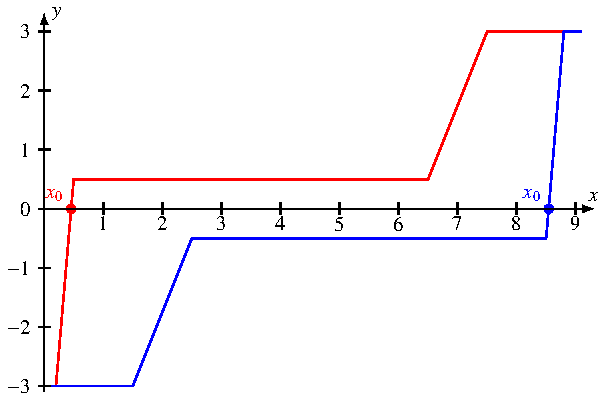
\includegraphics[width=\hsize]{../../buch/chapters/20-gleichungen/figures/stufe.pdf}
\end{center}
\end{column}
\end{columns}
\end{frame}
